\documentclass[a4paper]{article}
\usepackage{cmap}
\usepackage{mathtext}
\usepackage{amssymb}
\usepackage{amsmath}
\usepackage[russian]{babel}
\usepackage{indentfirst}
\usepackage[pdftex]{graphicx}
\usepackage{multirow}
\usepackage{mathrsfs}
\usepackage{biblatex}
\usepackage{siunitx}
\usepackage[left=2cm,right=2cm,top=2cm,bottom=2cm]{geometry}
\usepackage{fancyhdr}
\bibliography{bib}
\pagestyle{fancy}
\newcommand{\rref}[1]{(\ref{#1})}
\newenvironment{comment}{}{}
\newcommand{\picref}[1]{рис. \ref{#1}}
\newcommand{\mbf}{\mathbf}
\newcommand{\Equip}[3]{
	
	{\bf #1:} $\Delta = \pm #2$ \si{#3}}
\newcommand{\equip}[1]{
	
	{\bf #1}}
\newcommand{\labname}{Изучение дифракции света} 	% название пиши здесь
\newcommand{\labnum}{4.3.1}		% номер вводи здесь
\fancyfoot{}
\fancyhead[RE, RO]{\thepage}
\fancyhead[LE, LO]{Лабораторная работа \labnum \space \labname}
\title{Лабораторная работа \labnum \space \labname} % Название работы здесь
\author{Иван Сладков}
\begin{document}
\maketitle
\thispagestyle{empty}
\section{Аннотация}
В данной работе проводится исследование дифракции Френеля на щели и на препятствии, дифракции Фраунгофера на щели и на двух щелях; изучается влияние дифракции на качество изображений, даваемых оптическими приборами.

\section{Теоретические сведения}

\subsection{Дифракция Френеля на щели}

Распределение интенсивности света в плоскости наблюдения (см. \picref{fig:дифракцияФренеляУстановка}) проще всего рассчитывать с помощью зон Шустера. При освещении щели $ S_2 $ параллельным пучком лучей зоны Шустера представляют собой полоские, параллельные краям щели, изображённые на \picref{fig:ШустерЗоны}. 

\begin{figure}[tbp]
	\centering
	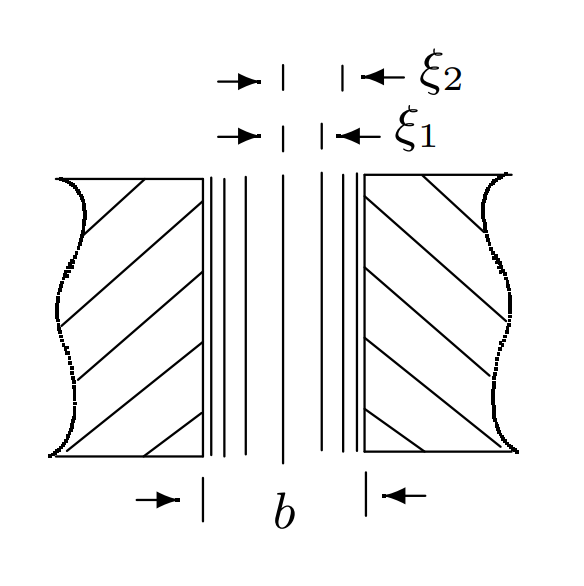
\includegraphics[width=0.5\linewidth]{Screenshot_1}
	\caption{Зоны Шустера, наблюдаемые при дифракции Френеля на щели}
	\label{fig:ШустерЗоны}
\end{figure}

Суммарная ширина $ n $ зон Шустера определяется соотношением:
\begin{equation}\label{eq:шустерзоны}
	\xi_n = \sqrt{n z \lambda},
\end{equation}
где $ \lambda $ -- длина волны; $ z $ -- расстояние между щелью и экраном.

Наблюдаемая на экране картина определяется волновым параметром:
\begin{equation}\label{eq:волновойПараметр}
	p = \frac{z \lambda}{b},
\end{equation}
где $ b $ -- толщина щели $ S_2 $. При $ p\ll 1 $ дифракция отсутствует (действует приближение геометрической оптики). При $ p\simeq 1 $ возникает дифракция Френеля с числом тёмных полос $ m $, тогда число зон на полуширине щели $ n = m+1 $.

Также можно ввести число Френеля, как число открытых зон на всей ширине щели:
\begin{equation}\label{eq:числоФренеля}
	C = \frac{b^2}{z \lambda} = \frac{1}{p^2}.
\end{equation}

\subsection{Дифракция Фраунгофера на щели}

При $ C\ll 1  $ наблюдается дифракция Фраунгофера с характерным распределением интенсивностей (см \picref{fig:Фраунгофер}). 

В центре поля зрения наблюдается дифракционный максимум. При малых углах $ \theta $ положение минимумов определяется соотношением:
\begin{equation*}\label{key}
	\theta_m = \frac{m \lambda}{b}.
\end{equation*}
Тогда расстояние от тёмной полосы до оптической оси $ O_2 $ равно:
\begin{equation}\label{eq:ФраунгоферМинимумы}
	x_m = m \frac{\lambda}{b} f_2,
\end{equation}
где $ f_2 $ -- фокус объектива.

\subsection{Дифракция Фраугофера на двух щелях}

Угловая координата $ \theta_m $ интерференционного максимума $ m $-го порядка определяется соотношением:
\begin{equation*}\label{key}
	\theta_m = \frac{m \lambda}{d},
\end{equation*}
где $ d $ -- расстояние между щелями. Тогда линейное расстояние между соседними интерференционными полосами равно:
\begin{equation}\label{eq:ИнтерфПолосыФраунгоф2}
	\delta x = \frac{\lambda}{d} f_2.
\end{equation}

Оценим число интерференционных полос в главном максимуме из соображений, что распределение интенсивностей такое же, как у одиночной щели (изображено пунктирной линией на \picref{fig:Фраунгофер3}):
\begin{equation}\label{eq:числоЛиний}
	n = \frac{2 \lambda f_2}{b} \frac{1}{\delta x} = \frac{2 d}{b}.
\end{equation}

\begin{figure}[tbp]
	\centering
	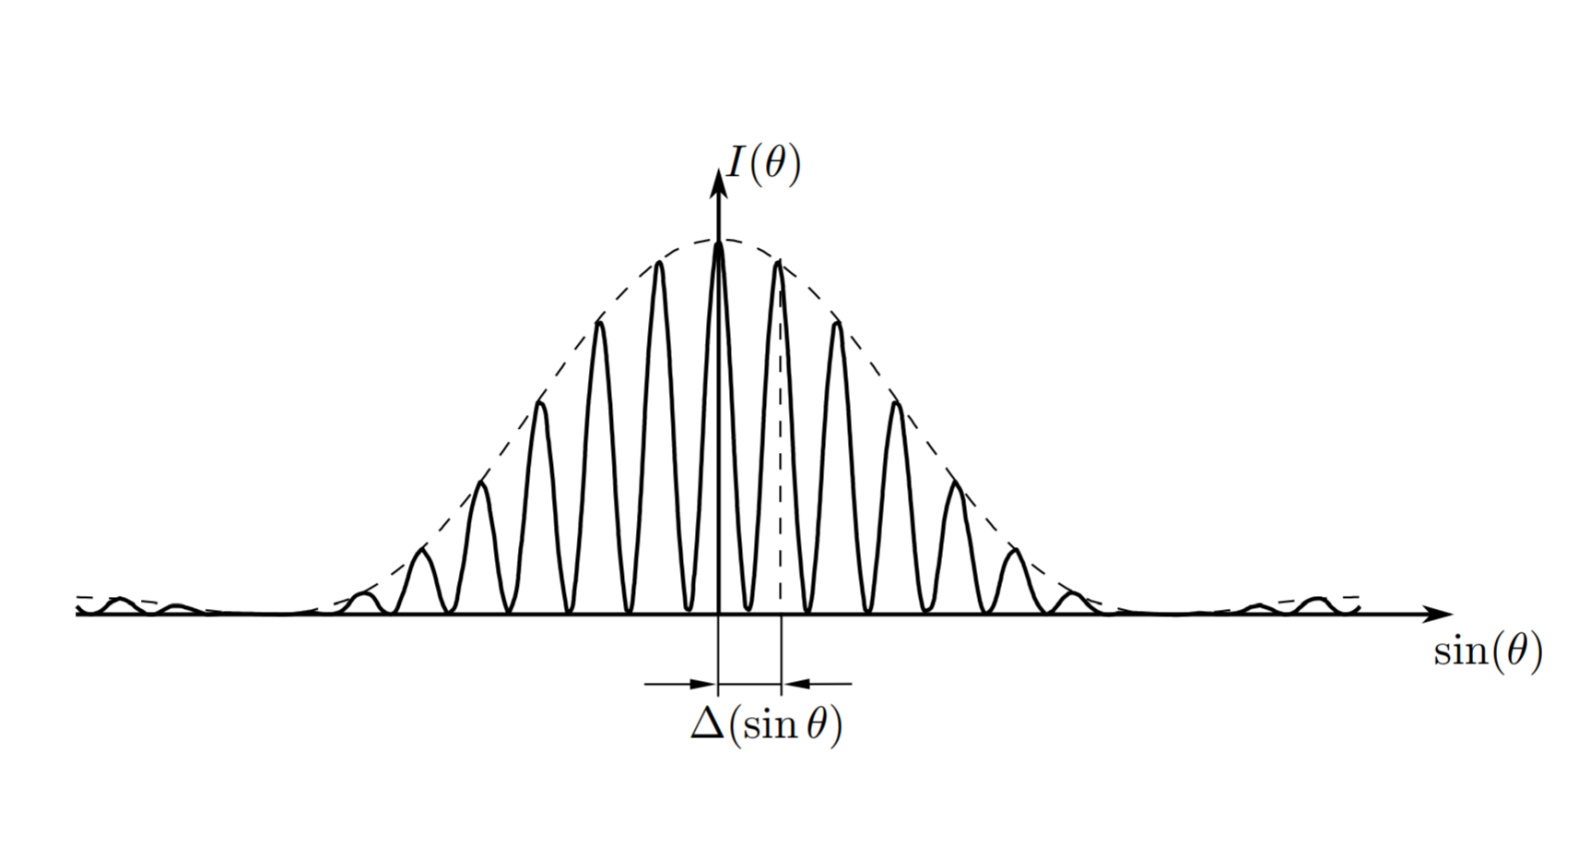
\includegraphics[width=0.8\linewidth]{Screenshot_5}
	\caption{Распределение интенсивностей в опыте с двумя щелями}
	\label{fig:Фраунгофер3}
\end{figure}


Для наблюдения интерференции требуется выполнение условия:
\begin{equation*}\label{eq:условиесрадиусом}
	d\le \rho_{ког} = \frac{\lambda}{b} f_1,
\end{equation*}
где $ \rho_{ког} $ -- радиус когерентности, $ b / f_1 $ -- угловая ширина входной щели $ S_1 $.

\subsection{Влияние дифракции на разрешающую способность оптического инструмента}

Установку на рис. \ref{fig:послустановка} можно рассматривать как оптический прибор. Для выявления его предельной разрешающей способности (ограниченной дифракцией на щели $ S_2 $) применяют критерий Рэлея:
\begin{equation}\label{eq:рэлей}
	\frac{\lambda}{D_0} = \frac{l}{f_2} = \frac{d}{f_1},
\end{equation}
где $ D_0 $ -- ширина щели $ S_0 $, $ l $ -- расстояние между изображениями щелей, $ d $ -- расстояние между щелями.

\section{Оборудование и инструментальные погрешности}

\equip{Микроскоп на поперечных салазках с микрометрическим винтом}: $ \Delta_{винта} = \SI{1}{\micro \metre}; \;\; \Delta_{шкалы} = \SI{0.02}{\milli \metre} $
\equip{Светофильтр}: $ \lambda = \SI{5461}{\angstrom}$
\equip{Щели с регулируемой шириной}: $ \Delta = \SI{1}{\micro \metre} $
\equip{Оптическая скамья}
\equip{Ртутная лампа}
\equip{Рамка с вертикальной нитью}
\equip{Двойная щель}
\equip{Зрительная труба}

Установки, применяемые в опыте, изображены на рис. \ref{fig:дифракцияФренеляУстановка}, \ref{fig:Фраунгофер}, \ref{fig:Фраунгофер2}, \ref{fig:послустановка}. Различия между установками для исследования дифракции Френеля и Фраунгофера состоят в том, что во втором случае необходимо поставить объектив $ O_2 $, чтобы приблизить исследуемую плоскость, на которой происходит дифракция.

\begin{figure}[tbp]
	\centering
	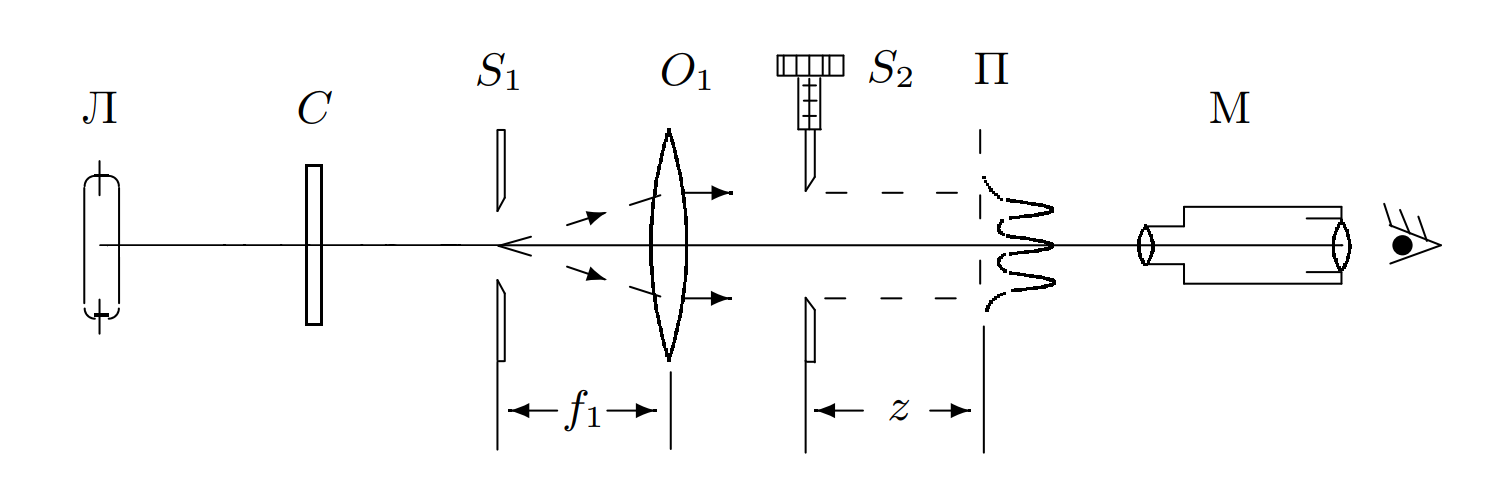
\includegraphics[width=0.8\linewidth]{Screenshot_2}
	\caption{Установка для наблюдения дифракции Френеля на щели}
	\label{fig:дифракцияФренеляУстановка}
\end{figure}


\begin{figure}[tbp]
	\centering
	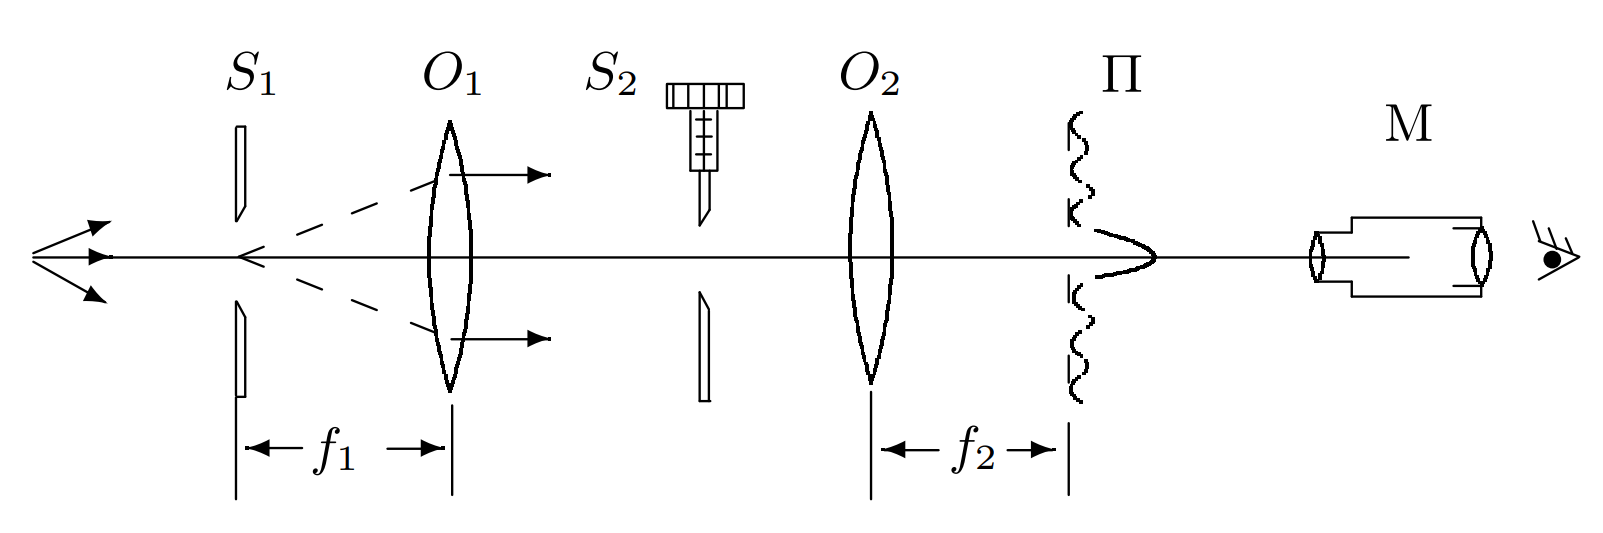
\includegraphics[width=0.8\linewidth]{Screenshot_3}
	\caption{Установка для наблюдения дифракции Фраунгофера на щели}
	\label{fig:Фраунгофер}
\end{figure}

\begin{figure}[tbp]
	\centering
	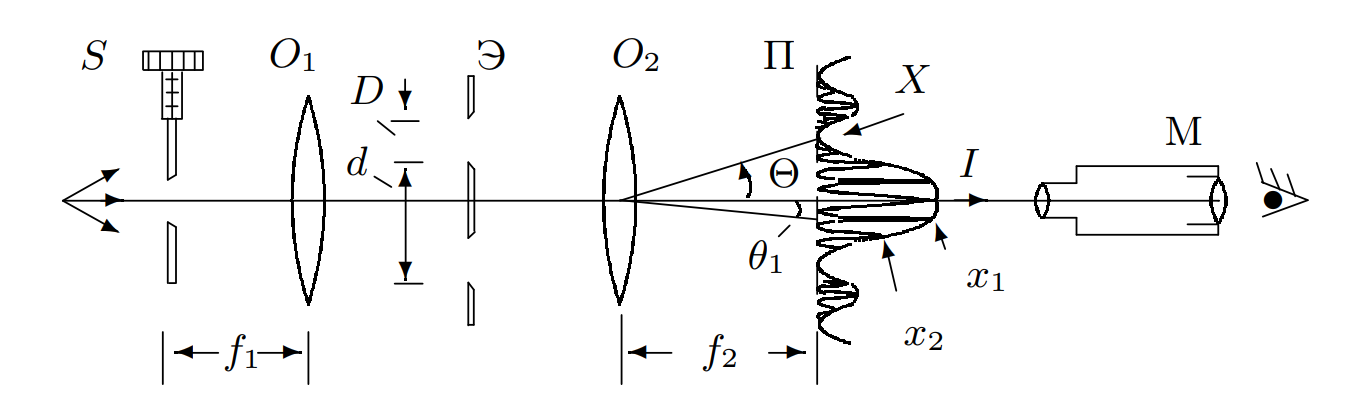
\includegraphics[width=0.8\linewidth]{Screenshot_4}
	\caption{Установка для наблюдения дифракции Фраунгофера на двух щелях}
	\label{fig:Фраунгофер2}
\end{figure}

\begin{figure}[tbp]
	\centering
	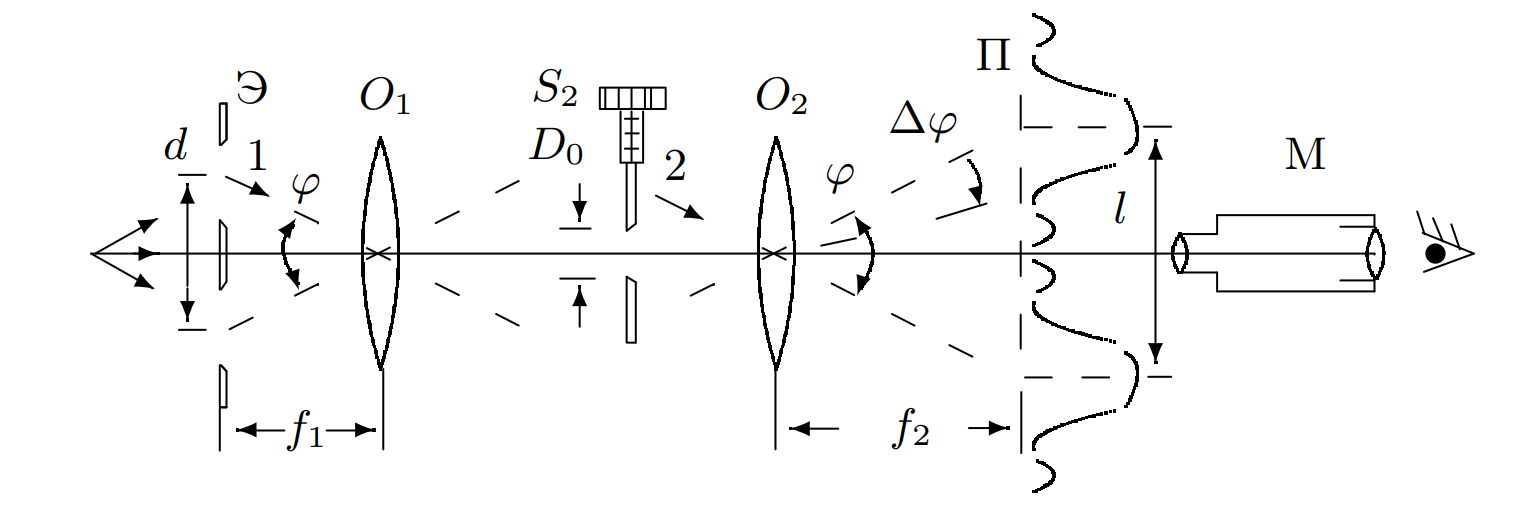
\includegraphics[width=0.8\linewidth]{Screenshot_9}
	\caption{Установка для исследования влияния дифракции на характеристики оптических приборов}
	\label{fig:послустановка}
\end{figure}


\section{Результаты измерений и обработка данных}
\emph{Все измерения и расчёты в СИ.}

\subsection{Дифракция Френеля на щели и препятствии}

\paragraph{Настройка.}

Найдём нуль микрометра на щели:
\begin{equation*}\label{key}
	 b_0 = 32 \pm 1 \; мкм.
\end{equation*}
Ширина щели по микрометрическому винту:
\begin{equation*}\label{key}
	b = 0.35 \pm 0.01 \; мм.
\end{equation*}
Методом последовательных приближений получим по возможности контрастную картину.

\paragraph{Измерения.}

Найдём начальное положение микроскопа (без дифракции):
\begin{equation*}\label{key}
	L_0 = 379 \pm 2\; мм.
\end{equation*}
Получим зависимость количества полос от расстояния в табл. 1: 
\begin{table}[h]
	\centering
	\begin{tabular}{|c|c|c|}
		\hline
		$m$ & $L, \; мм$ & $ z, \; мм $\\
		\hline
		1 & 409 & 30 \\
		\hline
		2 & 399 & 20 \\
		\hline
		3 & 394 & 15 \\
		\hline
		4 & 390 & 11 \\
		\hline
		5 & 388 & 9 \\
		\hline
		6 & 386 & 7 \\
		\hline
	\end{tabular}
	\label{tab:Френель}
	\caption{Зависимость количества тёмных полос от расстояния}
\end{table}
В этой таблице возьмём инструментальную погрешность $ \Delta = 2 \; мм $.
При помощи микрометрического винта на микроскопе и шкалы на окуляре найдём ширину щели:
\begin{equation*}\label{key}
	b^{микроскоп} = 0.34\pm 0.02 \; мм.
\end{equation*}
По микрометру на щели,
\begin{equation*}\label{key}
	b^{микрометр} = 0.35\pm 0.01 \; мм.
\end{equation*}
Значит, люфтом можно пренебречь.

\paragraph{Качественные наблюдения.}

При уменьшении щели уменьшается количество дифракционных полос. Это согласуется с теорией и обусловлено возрастанием волнового параметра \eqref{eq:волновойПараметр}.

Для дифракции Френеля на препятствии в виде тонкой вертикальной нити при удалении микроскопа -- чётное число тёмных полос.

\paragraph{Обработка данных.}

Сравним размер зон Шустера с шириной щели $ S_2 $. Построим график на рис. \ref{fig:ШустерГрафик}.
\begin{figure}[tbp]
	\centering
	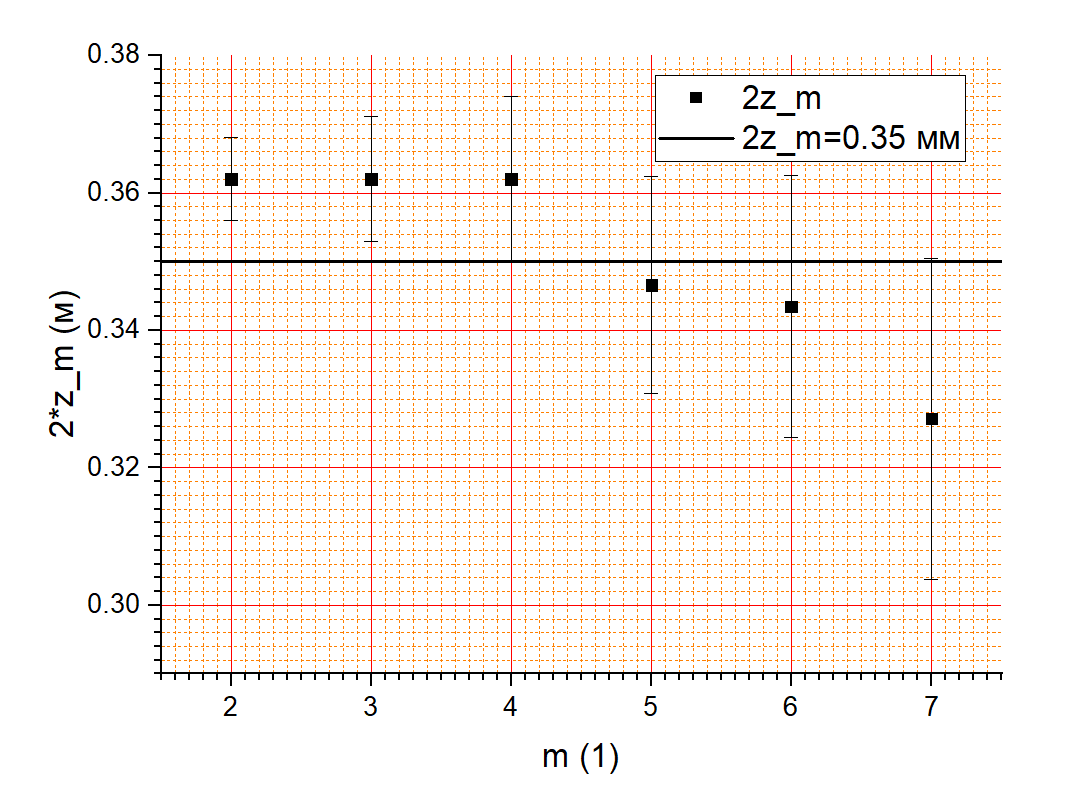
\includegraphics[width=0.8\linewidth]{Screenshot_6}
	\caption{Ширина зон Шустера}
	\label{fig:ШустерГрафик}
\end{figure}

\subsection{Дифракция Фраунгофера на щели}

\paragraph{Настройка.}

Фокус линзы-объектива $ O_2 $ равен $ 12.5\pm 0.1\; см $.
Получена дифракционная картина Фраунгофера на всё поле зрения микроскопа. 

\paragraph{Измерения.}

Снимем значения координат нескольких дифракционных минимумов в табл. 2.
\begin{table}[h]
	\centering
	\begin{tabular}{|c|c|c|c|c|}
		\hline
		$n$ & 1 & 2 & 3 & 4 \\
		\hline
		$X_m$ & 0.4 & 1.12 & 1.28 & 1.72 \\
		\hline
	\end{tabular}
	\label{tab:Фраунгофер}
	\caption{$ X_m (n) $ для опыта Фраунгофера }
\end{table}
Погрешность $ X_m $ в этой таблице считаем равной цене деления $ 0.02\; мм $. Ширина щели в этом опыте:
\begin{equation*}\label{key}
	b = 0.330 \pm 0.001 \; мм.
\end{equation*}

\paragraph{Качественные наблюдения.}

При смещении $ S_1 $ не происходит сдвига дифракционной картины. Это связано с тем, что картина находится в фокальной плоскости линзы $ O_2 $, куда приходят почти параллельные лучи.
При уменьшении ширины щели картина растягивается, что согласуется с формулой \eqref{eq:ФраунгоферМинимумы}.

\paragraph{Обработка данных.}

Построим график зависимости координаты $ X_m (n) $ на рис.\ref{fig:странныйграфик}.
\begin{figure}[tbp]
	\centering
	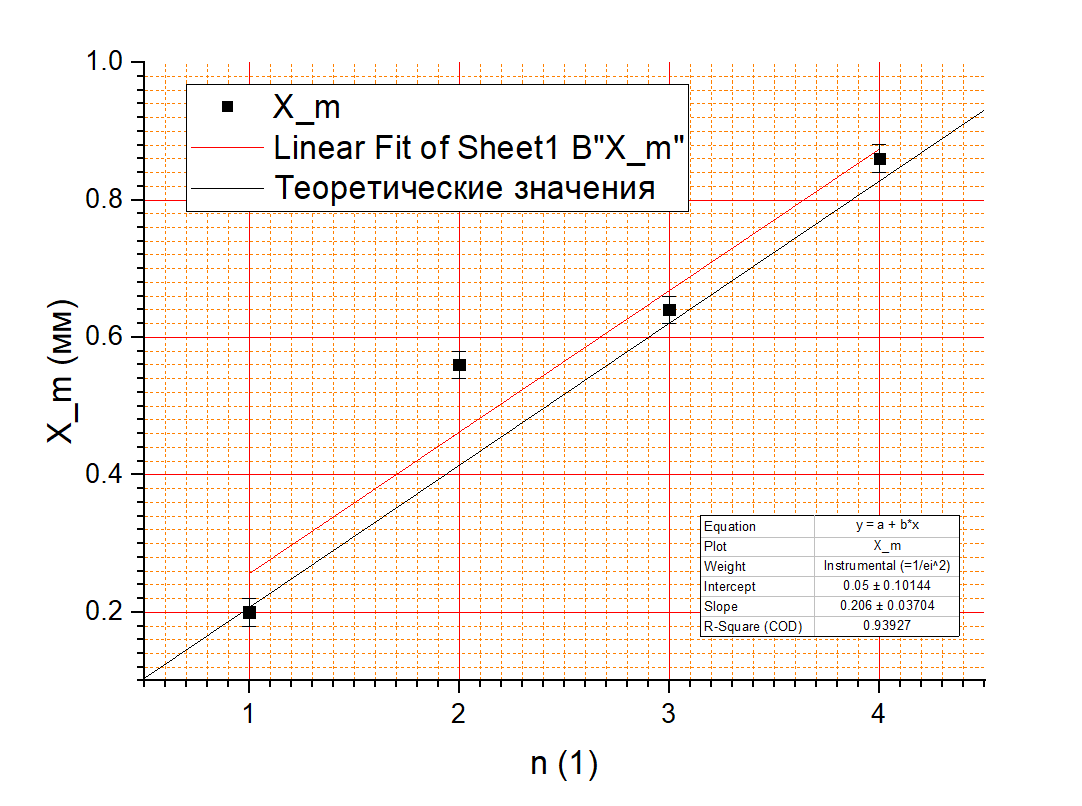
\includegraphics[width=0.8\linewidth]{Screenshot_8}
	\caption{Зависимость координаты минимума интенсивности от его номера}
	\label{fig:странныйграфик}
\end{figure}
Точки на графике довольно плохо сходятся к прямой, что может говорить о несовершенстве методики, или о том, что показания сняты неточно. Кроме того, точность результата уменьшается тем, что не была снята зависимость на отрицательных $ n $.
Поэтому результат
\begin{equation*}\label{key}
	\Delta X_m \approx 0.21\pm 0.04 \; мм
\end{equation*}
имеет сомнительную точность.
Расчётная $ X_m $ из \eqref{eq:ФраунгоферМинимумы} изображена на графике чёрной прямой, которая практически параллельна экспериментальной, как ни странно.

\subsection{Дифракция Фраунгофера на двух щелях}

\paragraph{Настройка и измерения.}

Получили по возможности чёткую дифракционную картину. Ширина центрального максимума при $ b=0.055\pm 0.001\; мм $ равна
\begin{equation*}\label{key}
	X = 2.00\pm 0.04 \;мм,
\end{equation*}
и он включает в себя $ n = 13 $ светлых промежутков.
Первое исчезновение интерференционных полос при
\begin{equation*}\label{key}
	b_0 = 0.16 \pm 0.01 \;мм.
\end{equation*}

\paragraph{Обработка результатов.}

Расстояние между минимумами равно:
\begin{equation*}\label{key}
	\delta x \approx \frac{X}{n} = 0.154\pm 0.003 \; мм.
\end{equation*}
Из формулы \eqref{eq:ИнтерфПолосыФраунгоф2}:
\begin{equation*}\label{key}
	d = \frac{\lambda f_2}{\delta x} = 0.45\pm 0.01.
\end{equation*}
Это значение отличается от замеренного: фактическое расстояние между щелями около $ 0.76\pm 0.02\; мм $. Расхождение может быть связано с неодинаковым расстоянием между щелями.

\subsection{Влияние дифракции на разрешающую способность оптического инструмента}

\paragraph{Настройка и измерения.}
Найдём минимальную ширину щели $ S_2 $, при которой изображения двух щелей ещё различимы:
\begin{equation*}\label{key}
	D_0 = 0.136\pm 0.001 \; мм.
\end{equation*}
Геометрические размеры щелей:
\begin{equation*}\label{key}
	d_1 = 0.14 \pm 0.02 \; мм,
\end{equation*}
\begin{equation*}\label{key}
	d_2 = 0.30 \pm 0.02 \; мм,
\end{equation*}
\begin{equation*}\label{key}
	d = 0.76 \pm 0.02 \; мм,
\end{equation*}
где $ d $ -- расстояние между щелями.

\paragraph{Обработка данных.}

Оценим выполнение критерия Рэлея. Из \eqref{eq:рэлей},
\begin{equation}\label{eq:last}
	D_0 = \frac{\lambda f_1}{d} = 0.08\pm 0.01\; мм.
\end{equation}
Значительное расхождение, вероятно, связано с субъективностью оценки <<щели всё ещё различимы>>. 

\subsection{Оценка погрешностей}

Везде в этой лабораторной оценки погрешностей проводились по схожему принципу: при обработке нескольких значений использовалась только статистическая погрешность, так как она существенно больше инструментальной. В остальных случаях аналитический расчёт погрешности проведён в \emph{Wolfram Mathematica}. Например, погрешность формулы \eqref{eq:last}:
\begin{equation*}\label{key}
	\sqrt{\frac{\lambda ^2\left((\delta x)^2 \sigma _{f_1}^2+f_1^2 \sigma _{\text{$\delta $x}}^2\right)}{(\delta x)^4}}.
\end{equation*}

\section{Вывод}

По результатам этой работы, изучили дифракцию Френеля и Фраунгофера. Провели сравнение установок, применяемых в этих опытах. Выявили различия этих двух явлений. Провели ряд сравнений значений, полученных экспериментально с расчётными. В нескольких случаях их несовпадения могут быть вызваны субъективностью визуальной оценки.

Исследовали влияние дифракции Фраунгофера на оптические приборы. Установили связь между уменьшением диафрагмы прибора и ухудшением разрешения, связанным с дифракцией.

С помощью качественных наблюдений установили ряд различий между исследуемыми явлениями и их особенности.

\newpage

\begin{thebibliography}{9}
	\bibitem{Siv} Сивухин Д. В. \emph{Общий курс физики. Том 4 Оптика}, 2004
	\bibitem{kir} Кириченко Н. А. \emph{Принципы оптики}, 2014
	\bibitem{max} \emph{Лабораторный практикум по общей физике. В 3 томах. Том 2. Оптика: учебное пособие} под ред. А. В. Максимычева
\end{thebibliography}
\end{document}